\documentclass[11pt, a4paper]{report}

\usepackage[T1]{fontenc}
\usepackage[utf8]{inputenc} 
\usepackage[english]{babel}
\usepackage[top=3cm, bottom=3cm, left=2cm, right=2cm]{geometry}
\usepackage{graphics}
\usepackage{graphicx}
\usepackage{eurosym}
\usepackage{soul}
\usepackage{graphicx} %utilisation d'images
\usepackage{amsmath}
\usepackage{relsize}
\usepackage{titlepic}


\begin{titlepage}
\newcommand*{\defeq}{\stackrel{\mathsmaller{\mathsf{def}}}{=}}
\title{Devoir de conception UML :\\Application de gestion des stages}
\author{GARCIA  Guillaume et ZAMBAUX Gauthier}
\date{\today}
\titlepic{
\includegraphics[scale=0.5]{Images/telecomnancy.png}

\includegraphics[scale=1]{Images/universitelorraine.jpg}}
\end{titlepage}

\begin{document}
\maketitle


\chapter*{Introduction}


\chapter*{Diagramme des classes}
\centerline{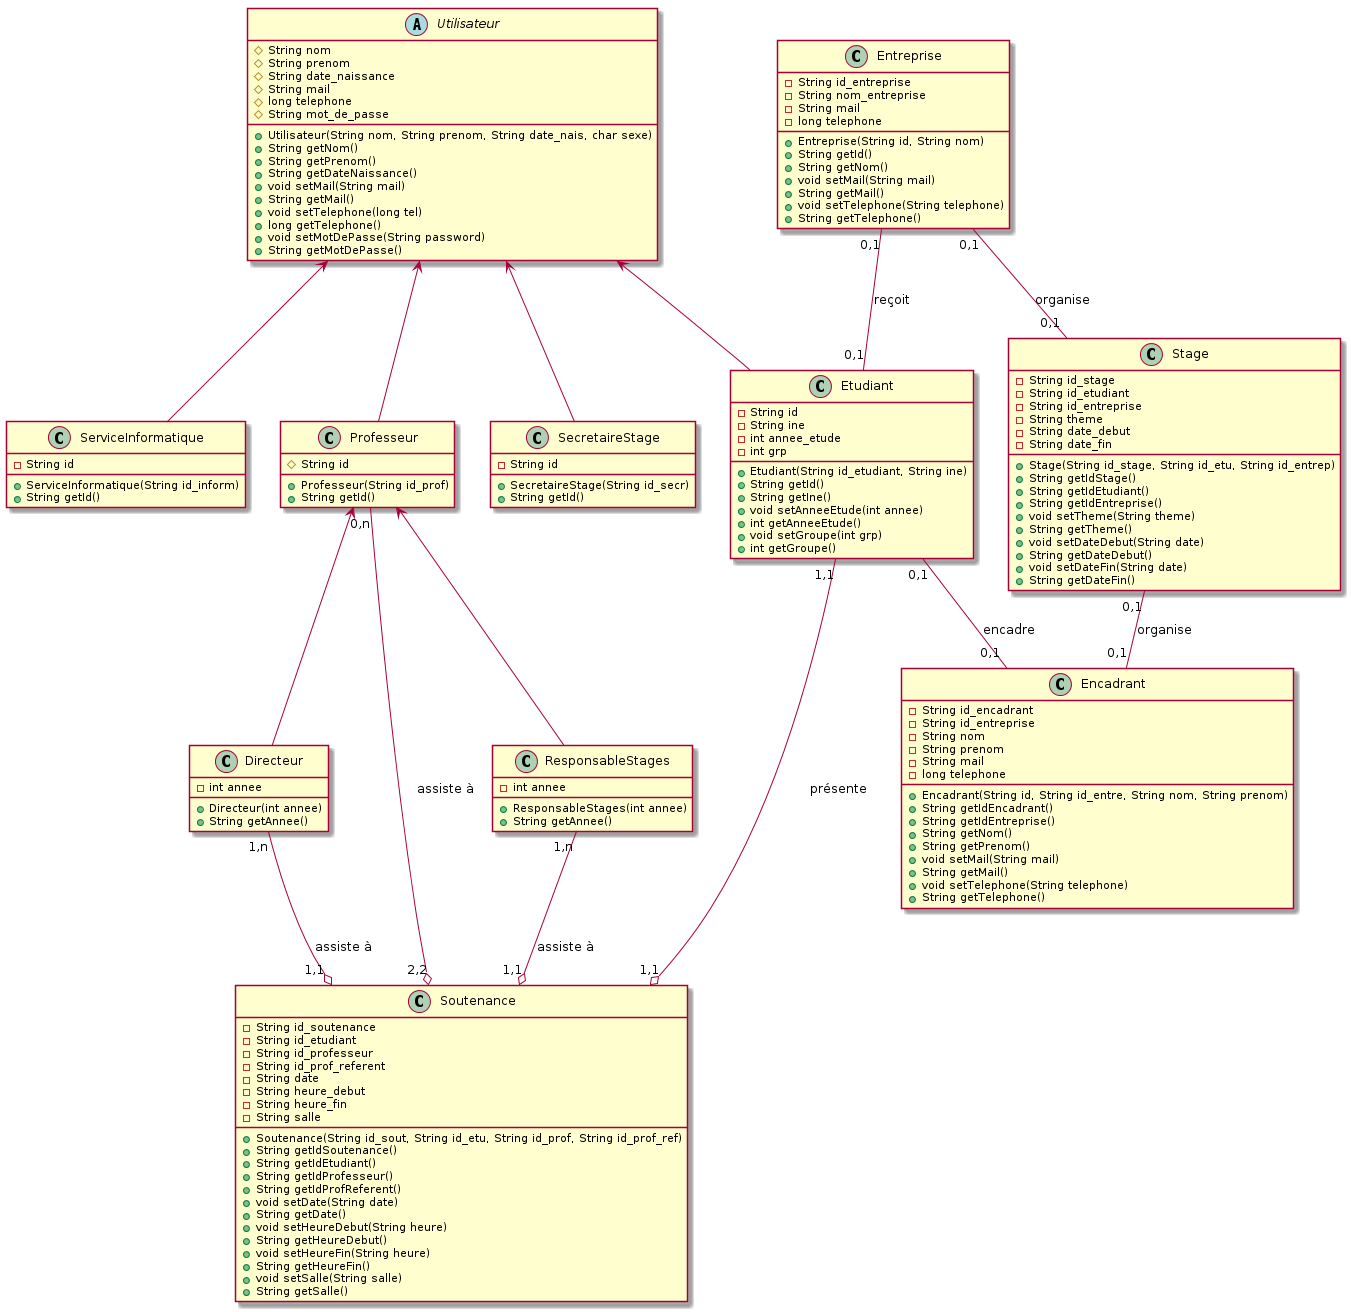
\includegraphics[scale=0.4]{Images/diagrammedesclasses.png}}


\chapter*{Diagrammes de séquence}

\section*{Saisie de la fiche de renseignements}
\centerline{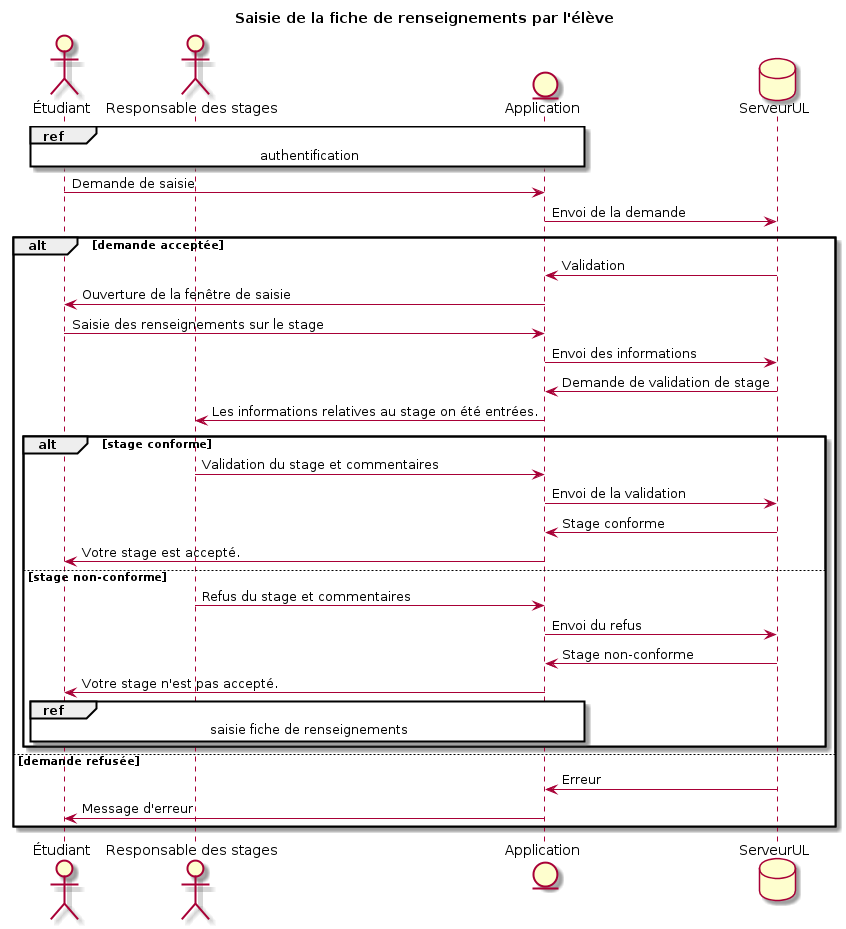
\includegraphics[scale=0.55]{Images/saisieficherenseignements.png}}

\section*{Prise de décision concernant une fiche de renseignements}
\centerline{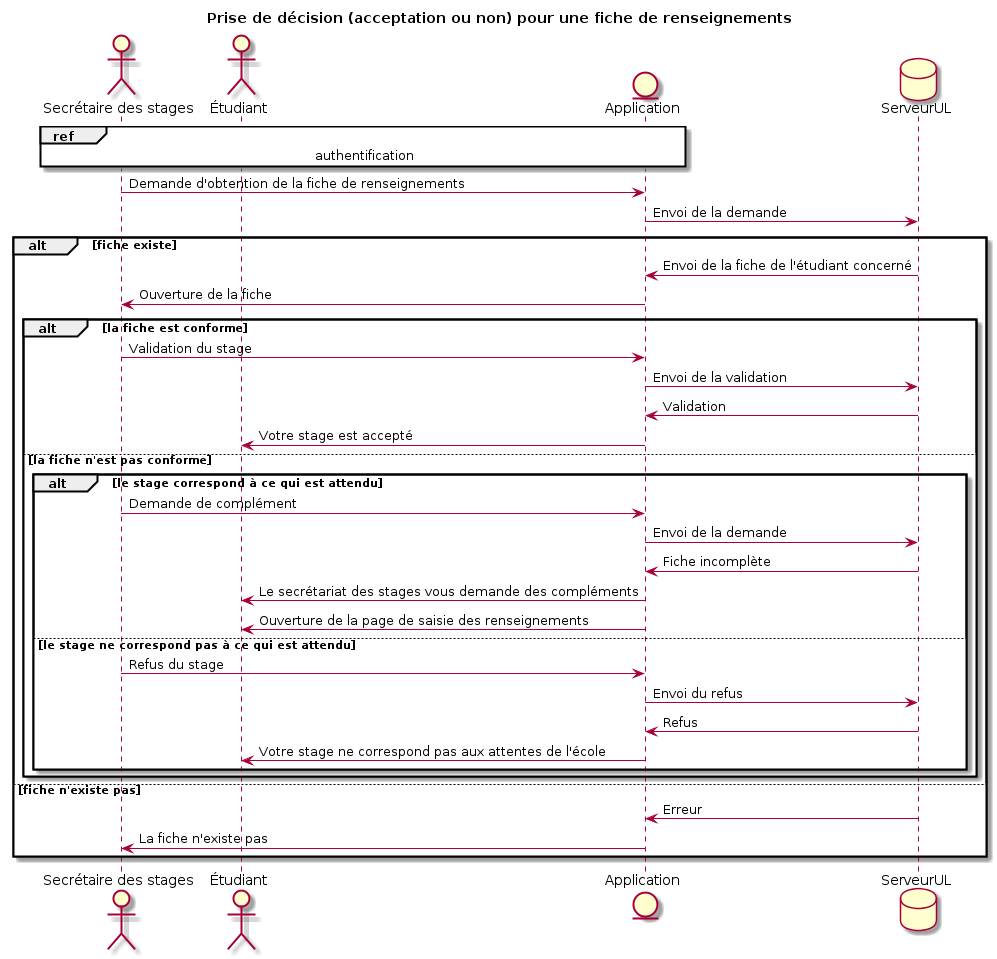
\includegraphics[scale=0.5]{Images/prisededecisionfichederenseignements.png}}
 
\section*{Initialisation d'une nouvelle année}
\centerline{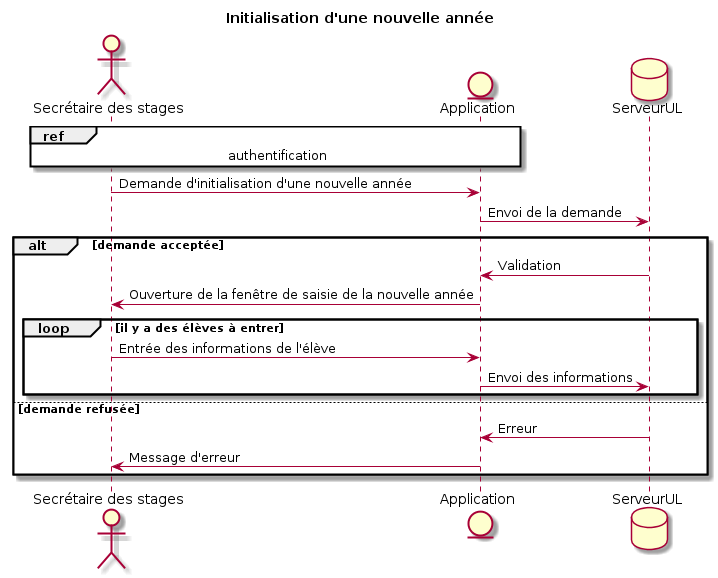
\includegraphics[scale=0.6]{Images/initialisationnouvelleannee.png}}


\chapter*{Diagramme d'états}
\centerline{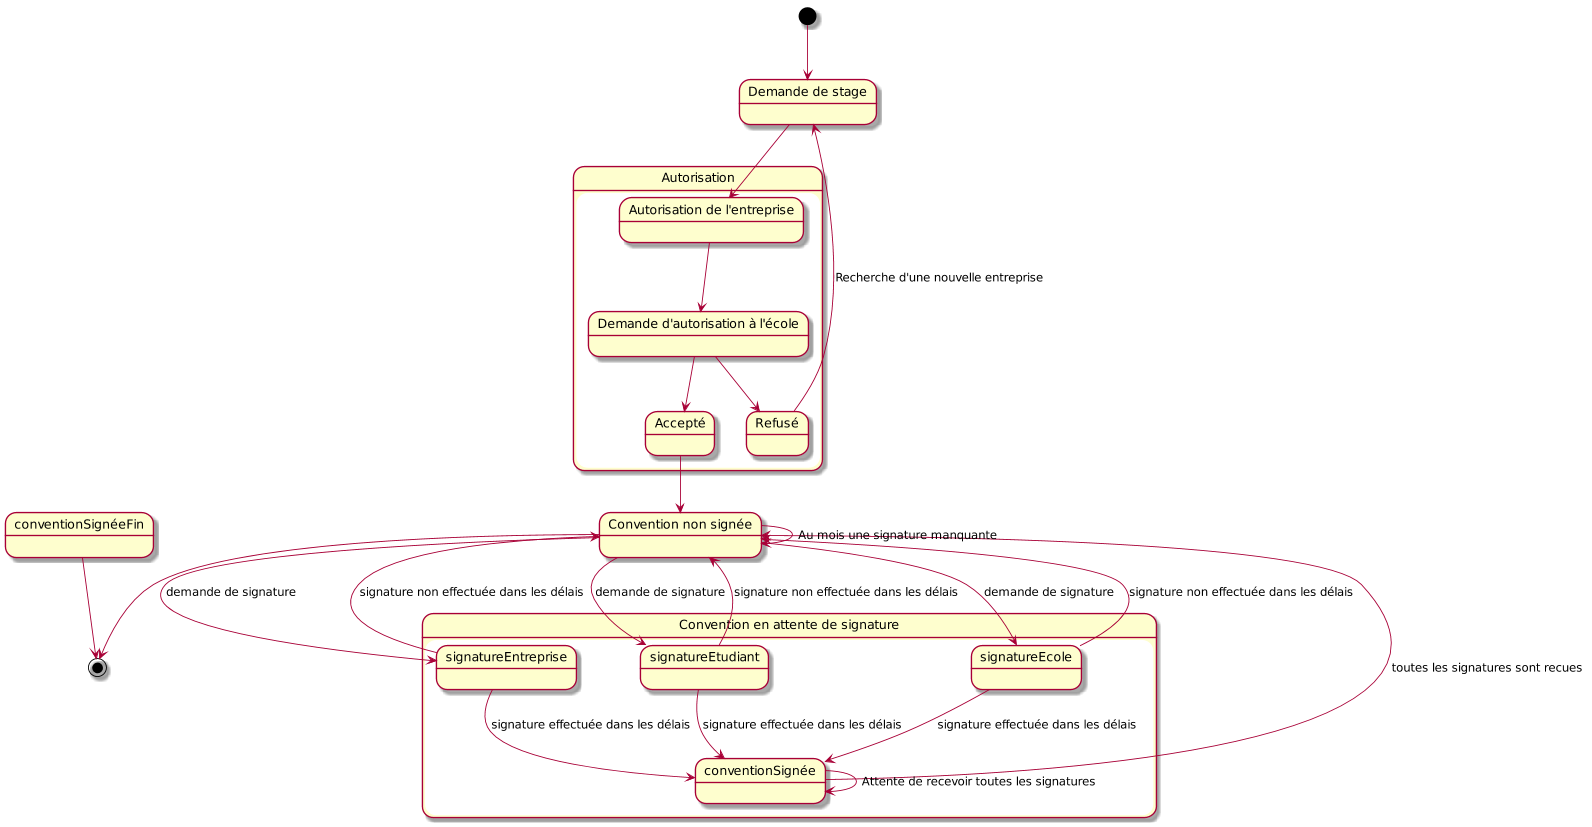
\includegraphics[scale=0.35]{Images/diagrammedetats.png}}


\appendix
\chapter*{Annexe A : Diagramme entités-associations}
\begin{center}
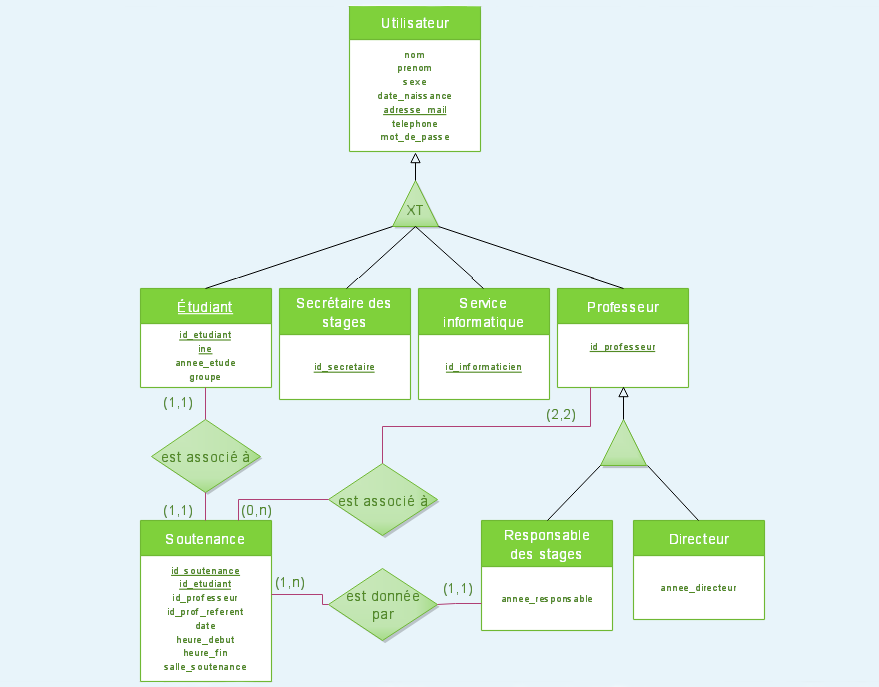
\includegraphics[scale=0.5]{Images/diagentiassoc.png}
\end{center}


\chapter*{Annexe B : Code UML des diagrammes}


\end{document}